\documentclass[a4paper, 12pt]{report}
\usepackage{cmap} % поиск в PDF
\usepackage[T2A]{fontenc} % Кодировка
\usepackage[utf8]{inputenc} % Кодировка исходного текста
\usepackage[english,russian]{babel} % Локализация и переносы
\usepackage{subcaption}
\captionsetup{compatibility=false}
\pagestyle{plain} % Для обозначения страниц справа снизу

\usepackage{graphicx}
\graphicspath{ {./images/} }

% Основная часть
\author{Автор: Булат Насыров}
\title{RFT\_CS \\ \footnotesize{\textit{Rocket fuel and trajectory computing system}}}
\date{\today}


\begin{document}
\maketitle

\tableofcontents{}
\clearpage
{\bfseries\Huge Предисловие}\\

\textrm{
    О чем будет идти речь, когда будем обсуждать ПО?\\
    Так же как любая метафора, описание программного обеспечения с точки зрения архитектуры может что-то скрыть, а что-то, наоборот, проявить; может обещать больше, чем давать, и давать больше, чем обещать. \\
    Оснавная привлекательность архитектуры - это структура. А структура - это то, что доминирует над парадигмами и суждениями в мире разработки ПО - компонентами, классами, функциями, модулями, слоями и службами, микро или макро. Но макроструктура многих программных систем часто пренебрегает убеждениями или пониманием - организация советских предприятий, невероятные небоскребы-башни (манареты) Дженга, достигающие облаков, археологические слои, залегающие в горной породе. Структура ПО не всегда интуитивно очевидна, как структура зданий.\\
    Здания имеют очевидную физическую структуру, независимо от материала, из которого они построены, от их высоты или ширины, от их назначения и от наличия или отсутствия архитектурных украшений. Их структура мало чем отличается - в значительной мере она обусловлена законом тяготения и физическими свойствами материалов. ПО, напротив, никак не связано с тяжестью, кроме чувства серьезности. И из чего же сделано ПО? В отличие от зданий, которые могут быть построены из кирпича, бетона, дерева, стали и стекла, программное обеспечение строится из меньших программных компонентов, и т.д., вплоть до основания.\\
    Говоря об архитектуре, можно сказать, что программное обеспечение по своей природе является фрактальным и рекурсивным, выгравированным и очерченным в коде. Здесь важные все детали. Переплетение уровней детализации также вносит свой вклад в архитектуру, но бессмысленно говорить о ПО в физических масштабах. Программное обеспечение имеет структуру - множество структур и множество их видов, - но их разнообразие затмевает диапазон физических структур, которые можно увидеть на примере зданий. Можно даже довольно убедительно утверждать, что при проектировании ПО архитектуре уделяется куда больше внимания, чем при проектировании зданий, - в этом смысле архитектура ПО является более многообразной, чем архитектура зданий!\\
    Но физический масштаб привычнее людям, и они часто ищут его в окружающем мире. Несмотря на привлекательность и визуальную очевидность, прямоугольники на диаграммах PowerPoint не являются архитектурой ПО. Да, они представляют определенный взгляд на архитектуру, значит не получить ни общей картины, ни понятия об архитектуре: архитектура ПО ни на что не похожа.
    Конкретный способ визуализации - не более чем частный выбор. Этот выбор основан на следующем наборе вариантов: что включить; что исключить; что подчеркнуть формой или цветом; что, наоборот, затенить. Никакой взгляд не имеет никаких преимуществ перед другим.\\
    Возможно, нет смысла говорить о законах физики и физических масштабах применительно к архитектуре ПО, но мы действительно учитываем некоторые физические ограничения. Скорость работы процессора и пропускная способность сети могут вынести суровый приговор производительности. Объем памяти и дискового пространства может ограничить амбиции любого программного кода. ПО можно сравнить с такой материей, как мечты, но ему приходится работать в реальном, физическим мире.
}

\chapter{Введение}
\section{Концепция}
\textrm{
    RFT\_CS (Rocket fuel and trajectory computing system) Система расчета ракетного топлива и траектории полета ракеты - это Python-библиотека для разработки математических моделей. RFT\_CS изначально был спроектирован так, чтобы его можно было внедрять постепенно. Другими словами, \textbf{вы можете начать с малого и использовать только ту функциональность RFT\_CS, которая необходима вам в данный момент}. Также в случае, если вам нужно изменить поведение/вычисления функции, есть возможность конфигурации методов под ваши нужды.
}
\section{Цель}
\textrm{
    Основная цель - создать математическую модель процессов, связанных с полётом одно и многоступенчатых, твердо и жидко топливных ракет и для вычисления траектории полёта баллистических ракет. Данное ПО может быть использовано для создания космических/баллистических ракет или своих научных экспериментов.
}
\section{Технологии}
\textrm{
    Программное обеспечение построено на высокоуровневом языке программирования Python и отдельные микропроцессоры написаны на языке C. Также для сложных математических вычислений использовались библиотеки, специально созданные для этой цели.
}
\clearpage

\section{Декомпозиция задачи}
\textrm{
    Начнём с составных частей ракеты, а также внешние факторы, влияющие на полёт. Начнём с состава космической ракеты:
}

\begin{figure}[!ht]
\centering
\begin{subfigure}
    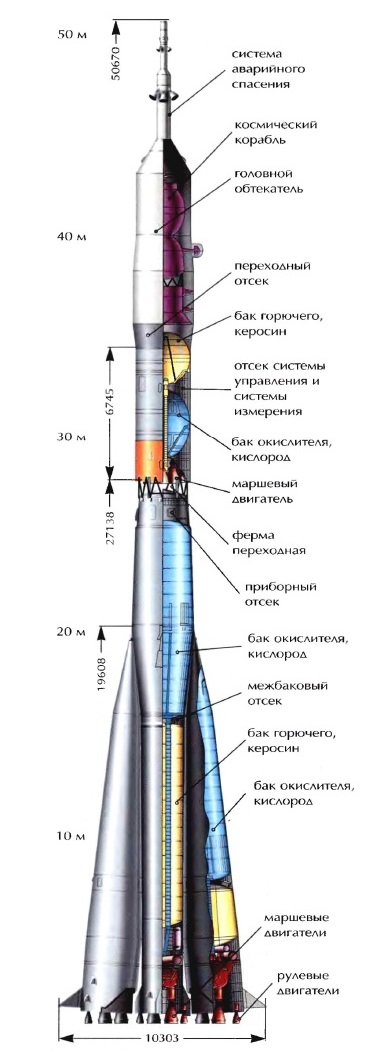
\includegraphics[width=.3\linewidth]{пример_космической_ракеты}
    \label{Рис. 1. Состав космической ракеты}
\end{subfigure}
\begin{subfigure}
    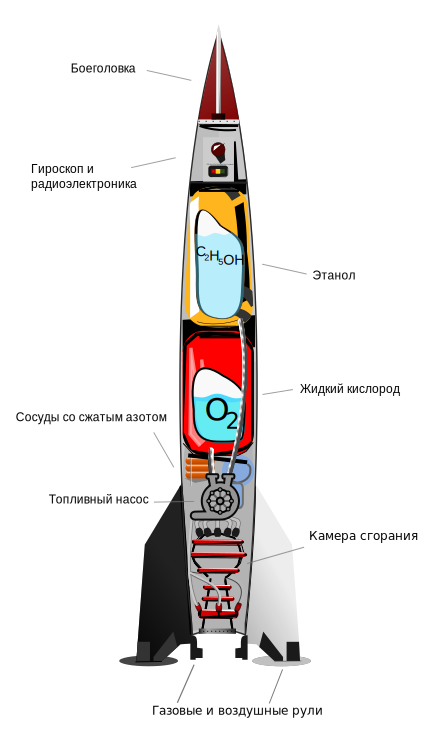
\includegraphics[width=.4\linewidth]{пример_баллистической_ракеты}
    \label{Рис. 2. Состав баллистической ракеты}
\end{subfigure}
\end{figure}

\section{Обработка ошибок}
\textrm{
    Могут возникать ошибки связанных с некорректным математических операций, перегрузкой или долгим ожиданием ответа от системы и неверным вводом/выводом данных, и др. Подобные ошибки обрабатываются и выводятся в виде ответа, а также записываются в логи. "{\bfseries При добавлении новых функций или использование встроенных функций важно не забывать обрабатывать ошибки и добавлять логирование для дальнейшего удобства исправления багов.}"
}
\clearpage

\end{document}

